\chapter{Ovládání}
Ovládání LED světel bylo zajištěno pomocí WiFi modulu, jenž součástí ESP32-DevKitC. Plánem bylo připojit mobilní telefon na WiFi modul a využít ho jako dálkový ovladač. 

Toho bylo dosáhnuto za pomoci aplikace RBController, což je aplikace speciálně Robotárnou navržena na řízení a ovládání desek za pomoci WiFi Modulu. Na Robotárně už se spoustu let využívá pro dálkové řízení robotů pomocí mobilních telefonů. Tato aplikace byla také použita na Letním Robotickém táboře 2020, který každoročně pořádá Helceletka.

Prvním krokem bylo si ale v aplikaci vytvořit a umístit tlačítka na řídící plochu tam, kde jsem je chtěla mít. A přesně k tomu jsem využila webovou aplikaci Esp32-RBGridUI-Designer, speciálně Robotárnou navrženou pro tuto práci


\section{\href{https://roboticsbrno.github.io/Esp32-RBGridUI-Designer/}{Esp32-RBGridUI-Designer}} 
Esp32-RBGridUI-Designer je webová aplikace, vytvořena Robotárnou za účelem navrhnutí ovládacího panelu, který se zobrazí v aplikaci RBController, při připojení uživatele k WiFi modulu. 

Webová aplikace dovoluje uživateli určit počet, barvu a umístění tlačítek na ovládacím panelu. Aplikace má příjemné prostředí a dobře se s ní pracuje. 

Webová stránka {\em Esp32-RBGridUI-Designer} má toto rozložení: 


\begin{figure}[htbp]
	\centering
	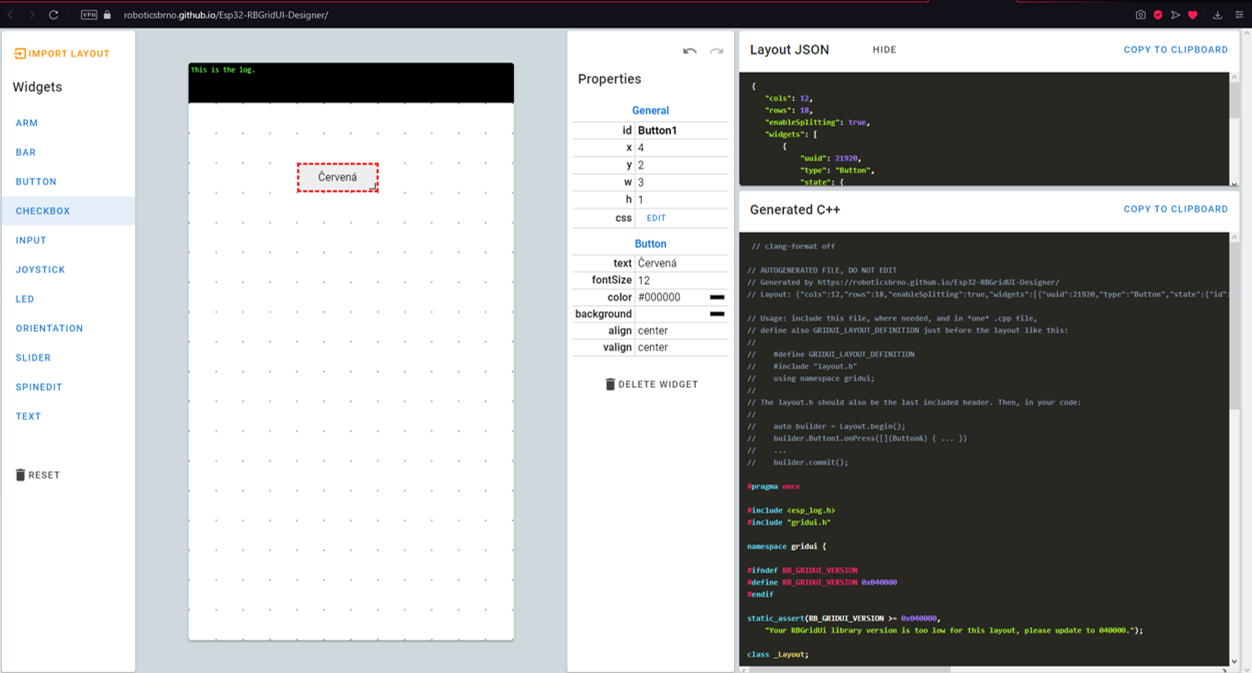
\includegraphics[width=1\textwidth]{img/Esp32-RBGridUI-Designer.png}
	\caption{Prostředí stránky {\em Esp32-RBGridUI-Designer}}
	%	\label{fig:install-sdk-3}
\end{figure}

\begin{enumerate}
	\item Postraní lišta, při kliknutí na jakoukoliv komponentu, je uživatel schopen danou kamponentu přetáhnout na manipulační plochu. 
	\item Manipulační plocha, na kterou se umisťují komponenty z postranní lišty. Nastavuje se tu jejich poloha a umístění. Manipulační plocha určuje vzhled řídící plochy v aplikaci v mobilním telefonu při napojení na daný Wifi modul. 
	\item  Tuto tabulku pro práci s ESP32-DevKitC potřebovat nebudeme.
	\item  Soubor Layout, který je potřeba stáhnout a nahrát do stejné složky jako máme hlavní program. Tento soubor nese informace toho, jakým způsobem jsme nanesli komponenty na manipulační plochu.
	\item Bližší specifikace, určující umístění, barvu, a název tlačítka, které bylo vytvořeno na~manipulační ploše. Tyto informace je možné zde i předělávat a upravovat.
	\item Tlačítko Reset které vymaže veškeré komponenty z Manipulační plochy a tím pádem i z Layoutu.
\end{enumerate}


% {\em Esp32-RBGridUI-Designer} je propojený s aplikací {\em RBControler,} \cite{RBControler}

\section{Vytvoření tlačítek - Jak se používá}
Plán byl vtvořit 4 různá tlačítka, která by přepínala mezi čtyřmi různě barevnými módy světla. Tyto tlačítka byla umístěna na ovládací plochu a přehledně pojmenována. 

Po vytvoření tlačítek v aplikaci, bylo důležité uložit text, který se nacházel v kolonce Layout JSON. Stačilo daný text zkopírovat a vložit do textového souboru layout.txt a příponu .txt přepsat na příponu .hpp. Pak bylo potřeba uchovat tento soubor pro budoucí užití.
\newpage


